La potencia eléctrica demandada por una vivienda modelo se ha extraído del
registro llevado por una comercializadora (Repsol) a través del área de
clientes de su página.

A pesar de no encontrarse disponible para descarga el histórico para un año
(solo se muestra de manera informativa un gráfico con el detalle por horas para
un día escogido), hemos podido rescatar esos datos a través de la API no
documentada de Repsol.

En la figura \ref{fig:repsol_api} se observa cómo en la carga de la página del
área de clientes se realiza una llamada al endpoint de la API
'hourly?date=20240825'.

\begin{figure}[h] \centering
	\centering
	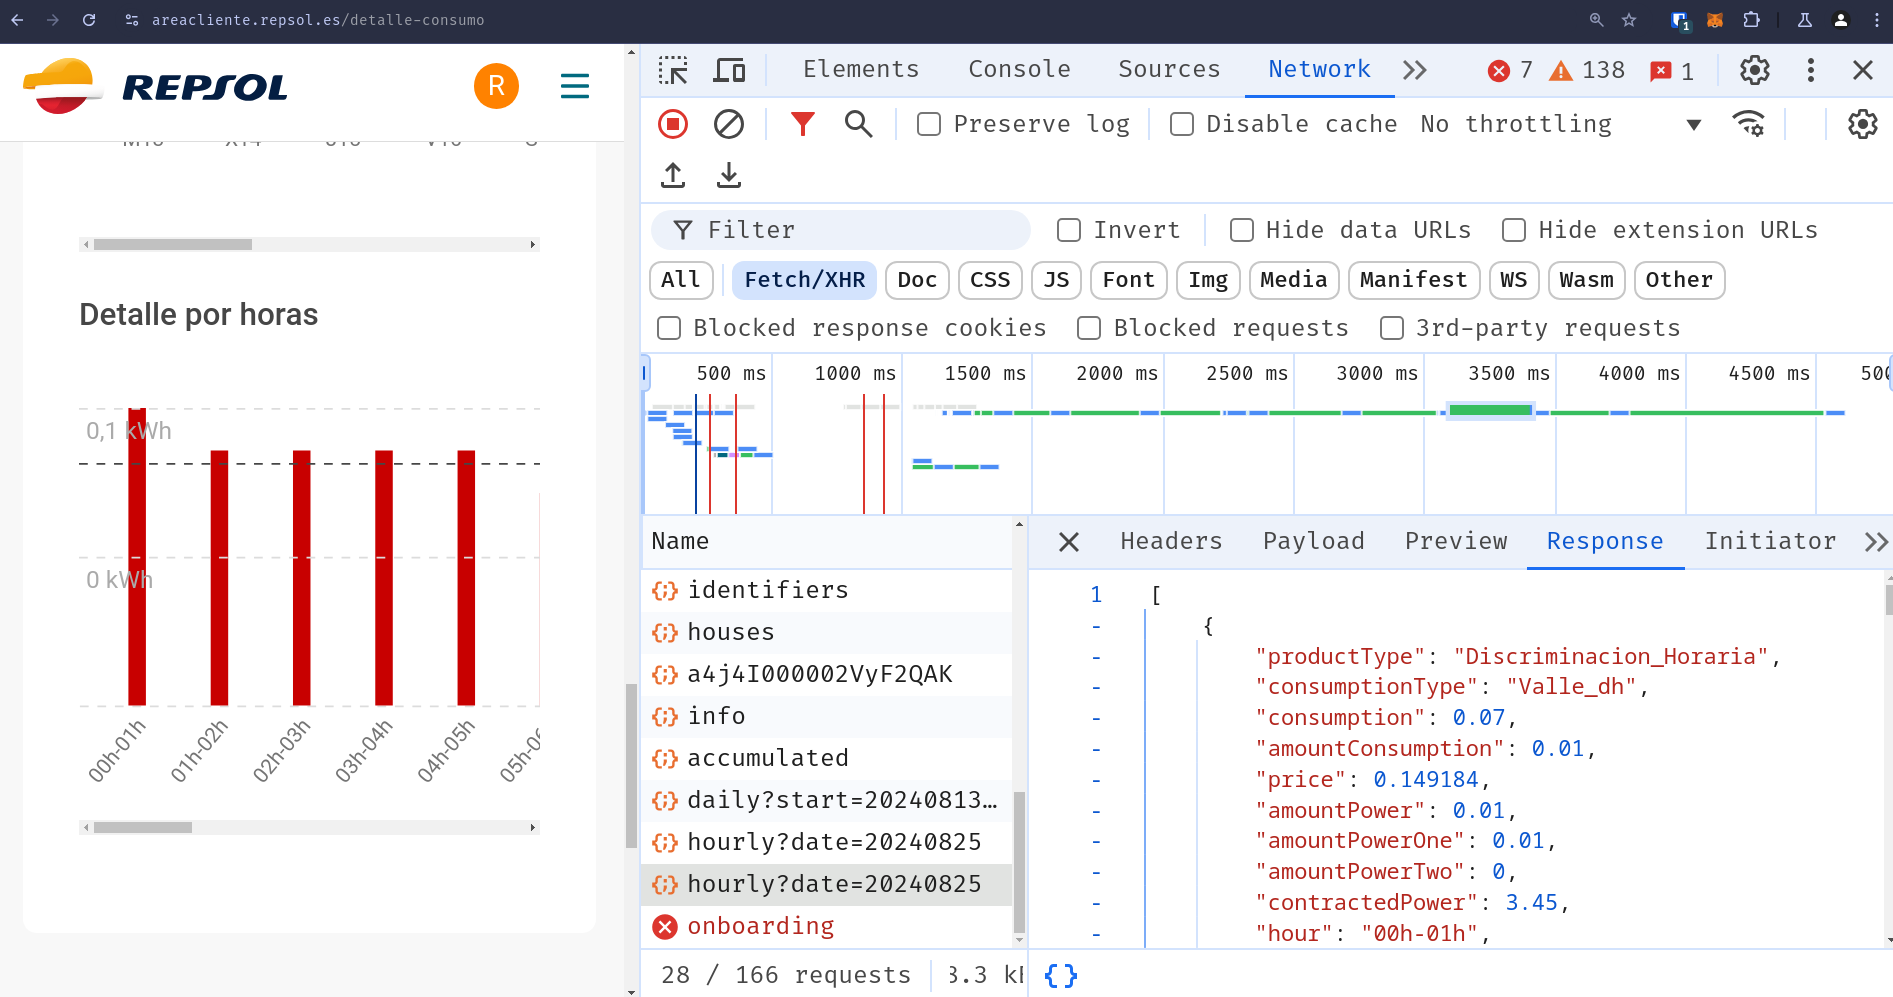
\includegraphics[width=1\textwidth]{./capitulos/adquisicion_de_datos/images/repsol_api.png}
	\caption{Llamada API para consumo horario en el área clientes de Repsol.}
	\label{fig:repsol_api}
\end{figure}

Con un pequeño script en javascript podemos reusar esa misma llamada, cambiando
tan solo la fecha del día, y así acumular los datos horarios para todo un año.

\begin{minted}{javascript}
async function fetchDataForDate(formattedDate) {
    const url = `https://areacliente.repsol.es/api/proxy/houses/a4j4I000002VyF2QAK/products/4302580717/consumption/hourly?date=${formattedDate}`;
    const requestParameters = {...}; // copied from real request
    const response = await fetch(url, requestParameters);
    const data = await response.json();
    return data;
}

const startDate = new Date('2023-01-01');
const endDate = new Date('2023-12-31');
const results = [];
for (let date = startDate; date <= endDate; date.setDate(date.getDate() + 1)) {
    let data = await fetchDataForDate(formattedDate);
    results.push(data);
}
\end{minted}

Para el año 2022 no se tienen registros, así que se han empleado los del 2023
(figura \ref{fig:p_demand_year}), pero se supone que la demanda eléctrica es
independiente del año escogido. La vivienda no dispone de aire acondicionado.

\begin{figure}[h] \centering
	\centering
	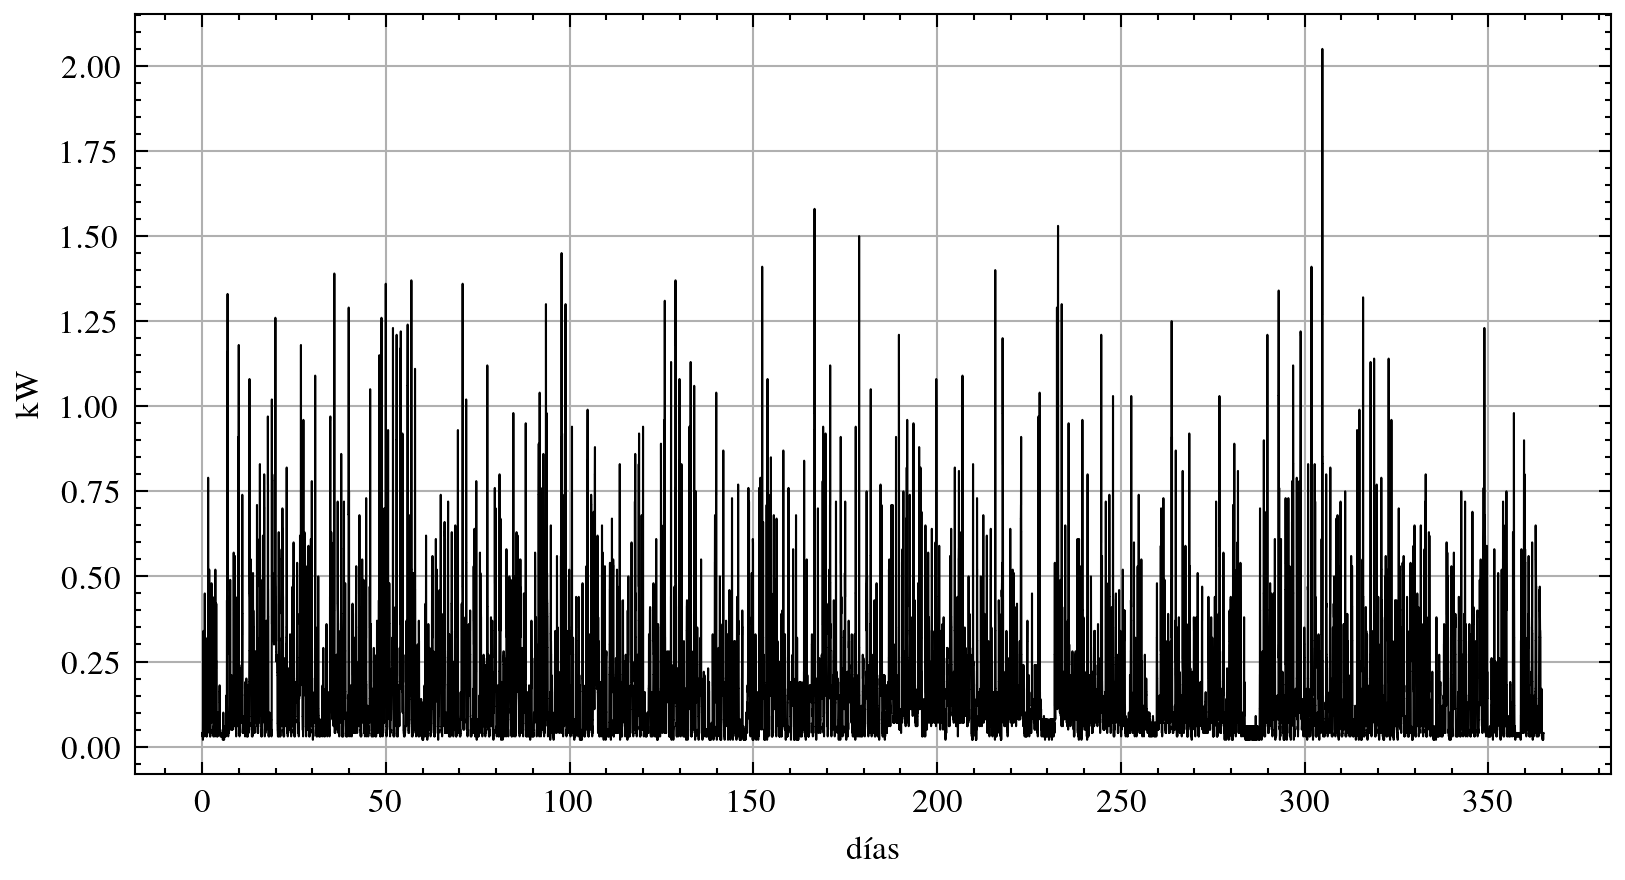
\includegraphics[width=1\textwidth]{./capitulos/adquisicion_de_datos/images/p_demand_year.png}
	\caption{Consumo eléctrico modelo para un año.}
	\label{fig:p_demand_year}
\end{figure}
